\begin{frame}{Bugs}

\emph{Discussion question}

  \begin{mycolumns}

    \begin{column}{.4\textwidth}\includegraphics[width=4in]{ch09/figs/parable-of-the-bugs.png}\end{column}

    \begin{column}{.6\textwidth}

      Before it was even cool, bug 1 got the idea of traveling along a straight path from A to B.
      Bug 2 does it too, but says he's being ironic.

      \vspace{2mm}

      Using our usual conventions, draw the spacetime diagram of both bugs' road trips, as bug 1 would choose
      to draw it.

      \vspace{2mm}

      How would it look if bug 2 drew it?

    \end{column}
  \end{mycolumns}

\end{frame}


\begin{frame}{The two-ton Timex}

\emph{Discussion question}

  \begin{mycolumns}

    \begin{column}{.3\textwidth}\includegraphics[width=3in]{ch09/figs/alley-plane-and-clock.jpg}\end{column}

    \begin{column}{.7\textwidth}

      The photos show a plane and set of atomic clocks used in a 1975-6 experiment by Alley \emph{et al.}.
      The clocks were flown aboard the plane, which
      circled at an altitude of 3000 meters above Chesapeake Bay for as long as possible without refueling.
      The clocks were then reunited with others that had stayed on the ground and compared with them.
      There is a special-relativistic effect because the plane is moving, and also a general-relativistic effect
      because the plane is up in the air. Would these two effects tend to reinforce one another, or would they
      partially cancel?

    \end{column}
  \end{mycolumns}


\end{frame}

\begin{frame}{Greatest time}

\emph{Discussion question}

      The figure shows two possible paths that a cannonball could take from event A to event B, with the
      ball drawn at intervals of a tenth of a second.

  \begin{mycolumns}

    \begin{column}{.3\textwidth}\includegraphics[width=3.25in]{ch09/figs/cannon-greatest-time.png}\end{column}

    \begin{column}{.7\textwidth}

      The principle of greatest time says that the ball should take the path that maximizes its own proper time.
      In each case, the ball's proper time will suffer a special-relativistic effect due to its motion,
      and also a general-relativistic effect because of its height.
      Discuss the directions of these effects and whether the results seem consistent with the principle of
      greatest time.

    \end{column}
  \end{mycolumns}

\end{frame}
